\section{Architectures' classification}

In 1966, Michael Flynn introduced a taxonomy outlining the architecture of calculators. 
This classification divides architectures into four categories:
\begin{itemize}
    \item \textit{Single Instruction Single Data}: utilized by uniprocessor systems.
    \item \textit{Multiple Instruction Single Data}: although theoretically possible, this architecture lacks practical configurations.
    \item \textit{Single Instruction Multiple Data}: features a straightforward programming model with low overhead and high flexibility, commonly employed in custom integrated circuits.
    \item \textit{Multiple Instruction Multiple Data}: known for its scalability and fault tolerance, this architecture is utilized by off-the-shelf microservices.
\end{itemize}

\subsection{Single instruction single data}
The traditional concept of computation involves writing software for serial execution, typically on a single computer with a lone Central Processing Unit (CPU).
Tasks are divided into a sequence of discrete instructions executed sequentially, allowing only one instruction to be processed at any given moment.
This arrangement is illustrated by the single instruction single data architecture.

\begin{figure}[H]
    \centering
    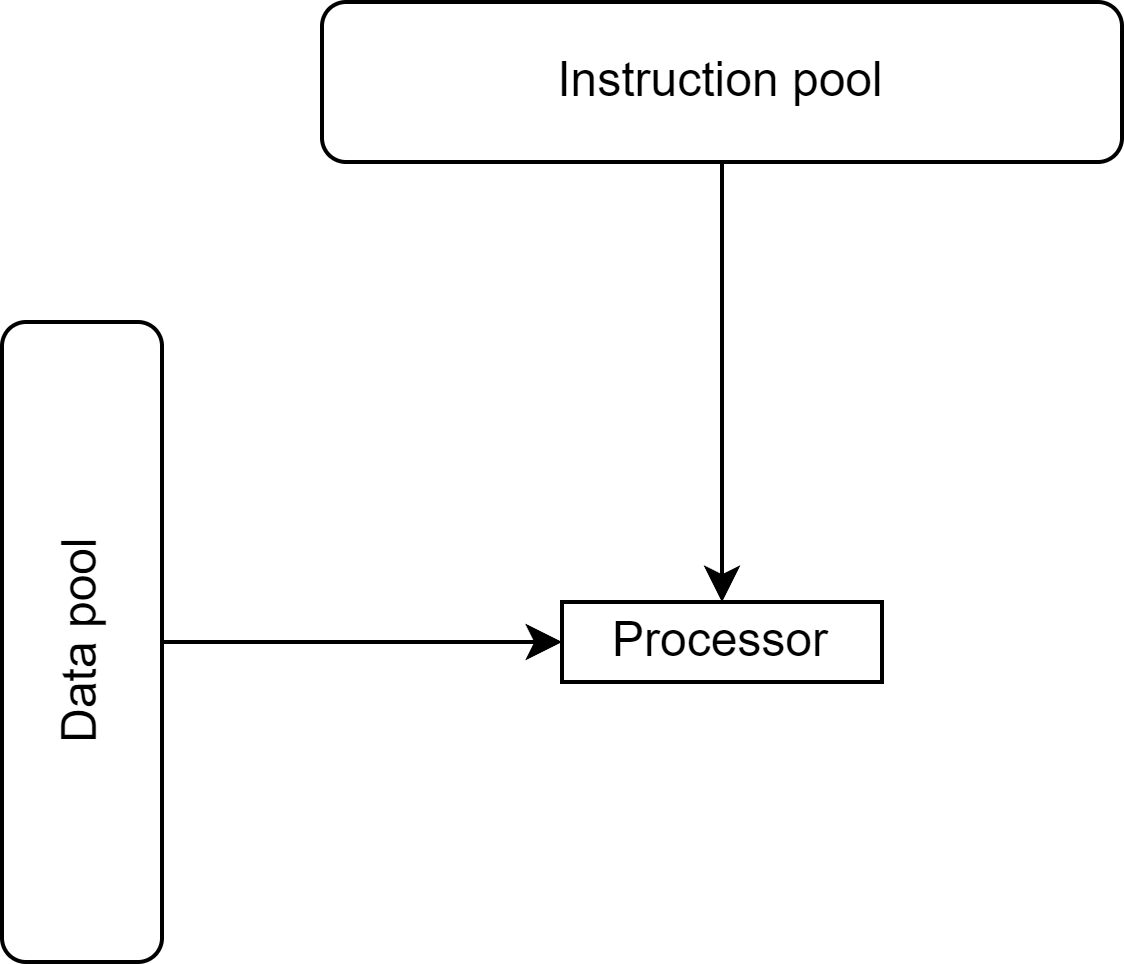
\includegraphics[width=0.3\linewidth]{images/sisd.png}
    \caption{Single Instruction Single Data (SISD)}
\end{figure}

In a single instruction single data architecture: 
\begin{itemize}
    \item \textit{Single instruction}: only one instruction is processed by the CPU in each clock cycle.
    \item \textit{Single data}: only one data stream is utilized as input during each clock cycle.
\end{itemize}
Execution in this setup is deterministic, meaning the outcome is predictable and follows a defined sequence of steps. 
Single instruction single data architecture architectures represent the most prevalent type of computers.

\subsection{Single instruction multiple data}
In the single instruction multiple data architecture, the following characteristics apply:
\begin{itemize}
    \item \textit{Single instruction}: all processing units execute the same instruction simultaneously during each clock cycle.
    \item \textit{Multiple data}: each processing unit can handle a different data element independently.
\end{itemize}
This architecture is particularly well-suited for specialized problems with a high level of regularity, such as graphics and image processing.

\begin{figure}[H]
    \centering
    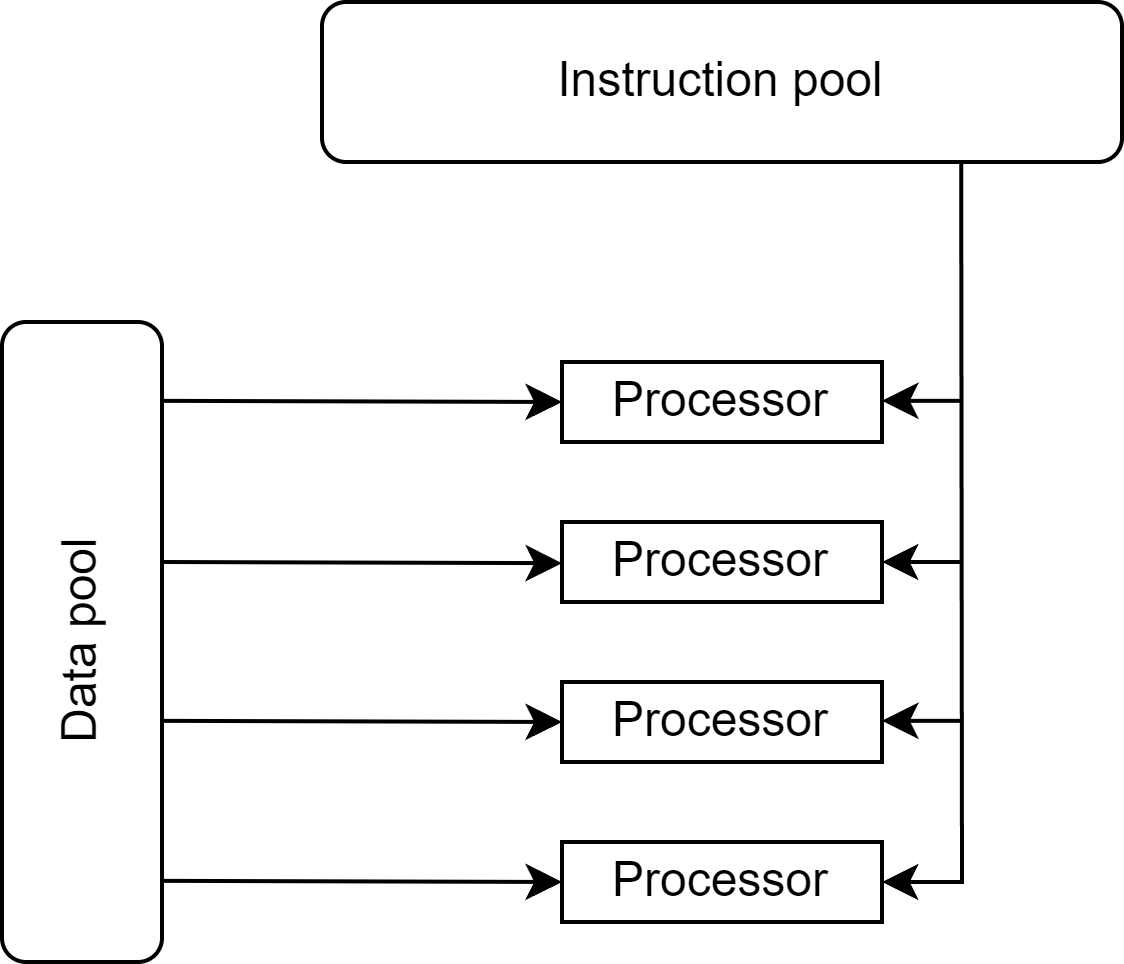
\includegraphics[width=0.3\linewidth]{images/simd.png}
    \caption{Single Instruction Multiple Data }
\end{figure}

\subsection{Multiple instructions architectures}
Hardware parallelism can be achieved through various methods:
\begin{itemize}
    \item \textit{Instruction-level parallelism}: this method harnesses data-level parallelism at different levels. 
        Compiler techniques such as pipelining exploit modest-level parallelism, while speculation techniques operate at medium levels of parallelism.
    \item \textit{Vector architectures and graphic processor units}: these architectures leverage data-level parallelism by executing a single instruction across a set of data elements simultaneously.
    \item \textit{Thread-level parallelism}: this approach exploits either data-level or task-level parallelism within a closely interconnected hardware model that enables interaction among threads.
    \item \textit{Request-level parallelism}: this method capitalizes on parallelism among largely independent tasks specified by either the programmer or the operating system.
\end{itemize}
Currently, the most common type of parallel computer features:
\begin{itemize}
    \item \textit{Multiple instruction}: each processor may execute a different instruction stream.
    \item \textit{Multiple data}: each processor may operate with a distinct data stream.
\end{itemize}
Execution in parallel computing can occur synchronously or asynchronously, and it may be deterministic or non-deterministic.

\begin{figure}[H]
    \centering
    \begin{subfigure}{0.49\textwidth}
        \centering
        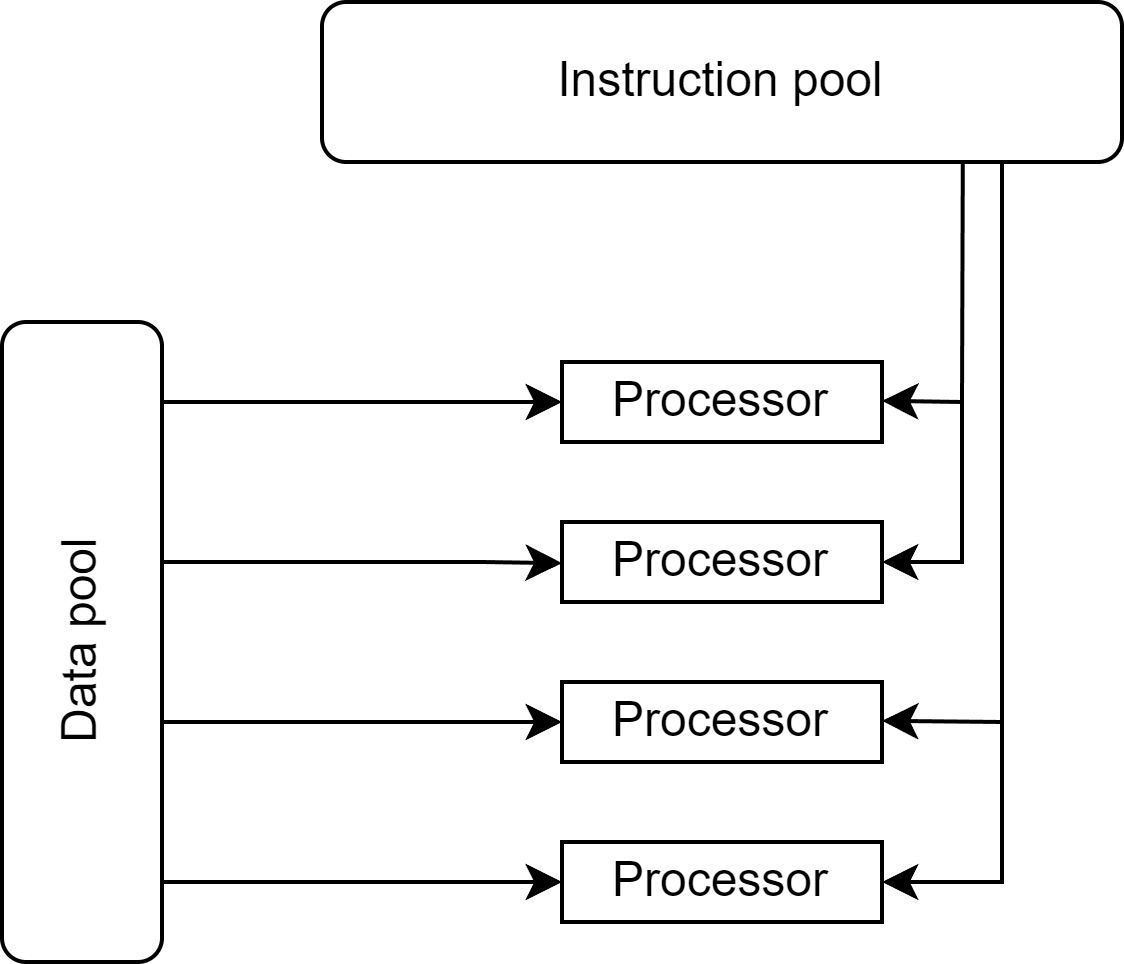
\includegraphics[width=0.6\linewidth]{images/mimd.png} 
        \caption{Multiple Instruction Multiple Data}
    \end{subfigure}
    \begin{subfigure}{0.49\textwidth}
        \centering
        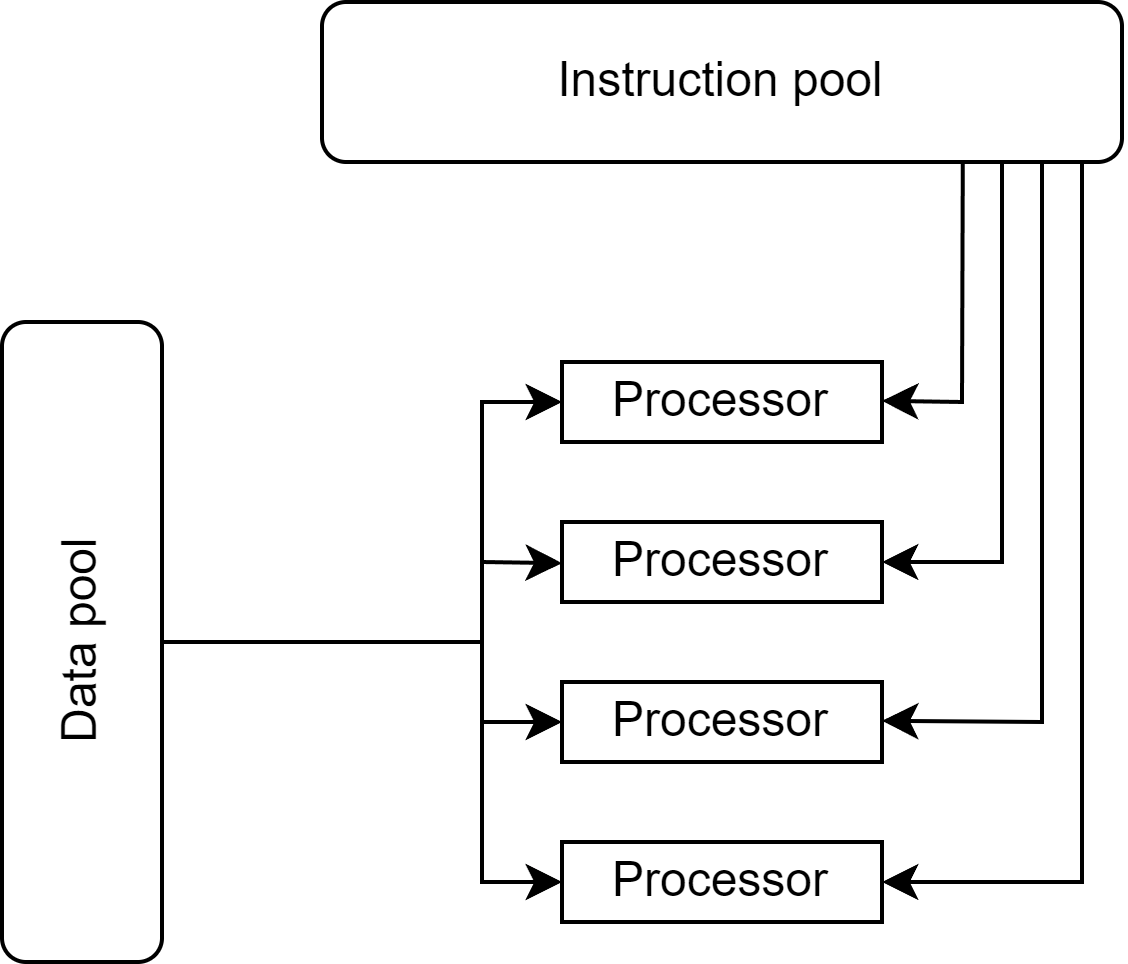
\includegraphics[width=0.6\linewidth]{images/misd.png}
        \caption{Multiple Instruction Single Data}
    \end{subfigure}
    \caption{Possible architectures for hardware parallelism}
\end{figure}